% %%%%%%%%%%%%%%%%%%%%%%%%%%%%%%%%%%%%%%%%%%%%%%%%%%%%%%%%%%%%%%%%%%%%%%
%  ╭─────────╮                      ╔══╦╗ ╗ ╔═╦═╗ ╥ ┌─┐┌─┐┌─┐┬ ┬┌─┐┌┐ ┬
%  │ ,-= ━━━┑│                  |   ╠═╦╝╚╗╠╗║ ║ ╠═╣ ├─┤├─┤│  ├─┤├─ │└┐│
%  │ % iTec  │                  |   ╨ ╚═ ╚╝╚╝ ╨ ╨ ╨ ┴ ┴┴ ┴└─┘┴ ┴└─┘┴ └┘
%  │┃°. .°.  │ Chair Individual |          ┬ ┬┌┐ ┬┬┬  ┬┌─┐┬─┐┌─┐┬┌┬┐┬ ┬
%  │┖  °   ° │   and Technology |          │ ││└┐││└┐┌┘├─ ├┬┘└─┐│ │ └┬┘
%  ╰─────────╯                             └─┘┴ └┘┴ └┘ └─┘┴└─└─┘┴ ┴  ┴
% %%%%%%%%%%%%%%%%%%%%%%%%%%%%%%%%%%%%%%%%%%%%%%%%%%%%%%%%%%%%%%%%%%%%%%
%  This file is part of the Master's thesis LaTeX template used at the
%  Chair Individual and Technology (iTec) at RWTH Aachen University.
% %%%%%%%%%%%%%%%%%%%%%%%%%%%%%%%%%%%%%%%%%%%%%%%%%%%%%%%%%%%%%%%%%%%%%%


%% %%%%%%%%%%%%%%%%%%%%%%%%%%%%%%%%%%%%%%%%%%%%%%%%%%%%%%%%%%%%%%%%%%%%%
\chapter{Results}
\label{chap:results} 

\section{Wilcoxon Signed-Rank Test for Face Validity}

To assess the face validity of the agents’ numeric opinions, the scores generated by the LLM agents were compared with those predicted by human annotators using the Wilcoxon Signed-Rank Test. This non-parametric test was chosen due to the ordinal nature of the 7-point Likert scale and the dependent (paired) design of the observations. A separate analysis was conducted for each questionnaire item. The results, including the test statistic ($\text{W}$), two-sided $p$-value, and Mean Absolute Error ($\text{MAE}$), are summarised in Table~\ref{tab:wilcoxon_results_bonferroni}.

\begin{table}[!htbp]
\centering
\caption{Wilcoxon Signed-Rank Test: Comparison of Agent and Annotator Scores, including Bonferroni Adjustment}
\label{tab:wilcoxon_results_bonferroni}
\begin{tabular}{l c c c c c}
\toprule
\textbf{Question} & $\mathbf{N}$ & $\mathbf{W}$ & $\mathbf{p\text{-value}}$ & $\mathbf{MAE}$ & $\mathbf{p_{\text{Bonferroni}}}$ \\
\midrule
Speed limit & 16 & $4.0$ & $0.013$ & $0.81$ & $0.063$ \\
Voting age 16 & 12 & $4.0$ & $0.125$ & $0.58$ & $0.625$  \\
Defense spending & 15 & $25.0$ & $0.791$ & $0.93$ & $1.000$ \\
Wind energy & 6 & $0.0$ & $0.250$ & $1.00$ & $1.000$ \\
Rent control & 11 & $12.0$ & $0.563$ & $0.82$ & $1.000$ \\
\bottomrule
\end{tabular}
\end{table}


For the majority of questionnaire items ($4$ out of $5$), there was no statistically significant difference between the agents’ scores and those predicted by human annotators. Specifically, the agents’ opinions on voting age, defence spending, wind energy, and rent control aligned closely with human expectations, indicating strong face validity.

A statistically significant difference was observed for the statement regarding a general speed limit on all motorways ($\text{W} = 4.0$, $p = 0.013$). However, after applying the Bonferroni adjustment ($p_{\text{Bonferroni}} = 0.063$), this result no longer reached the corrected significance threshold. Therefore, there is insufficient evidence to conclude a meaningful difference between human-annotated and LLM-generated scores for any of the questionnaire items.

To visualise the agreement between annotators and model outputs, Figure~\ref{fig:sanity_check} presents a paired dot plot. Each line connects the corresponding annotator and model ratings for a given questionnaire item, while darker colours indicate overlapping values. The plot illustrates that most paired ratings are closely aligned, suggesting limited deviation between human and model judgements.

\begin{figure}[!htbp]
\centering
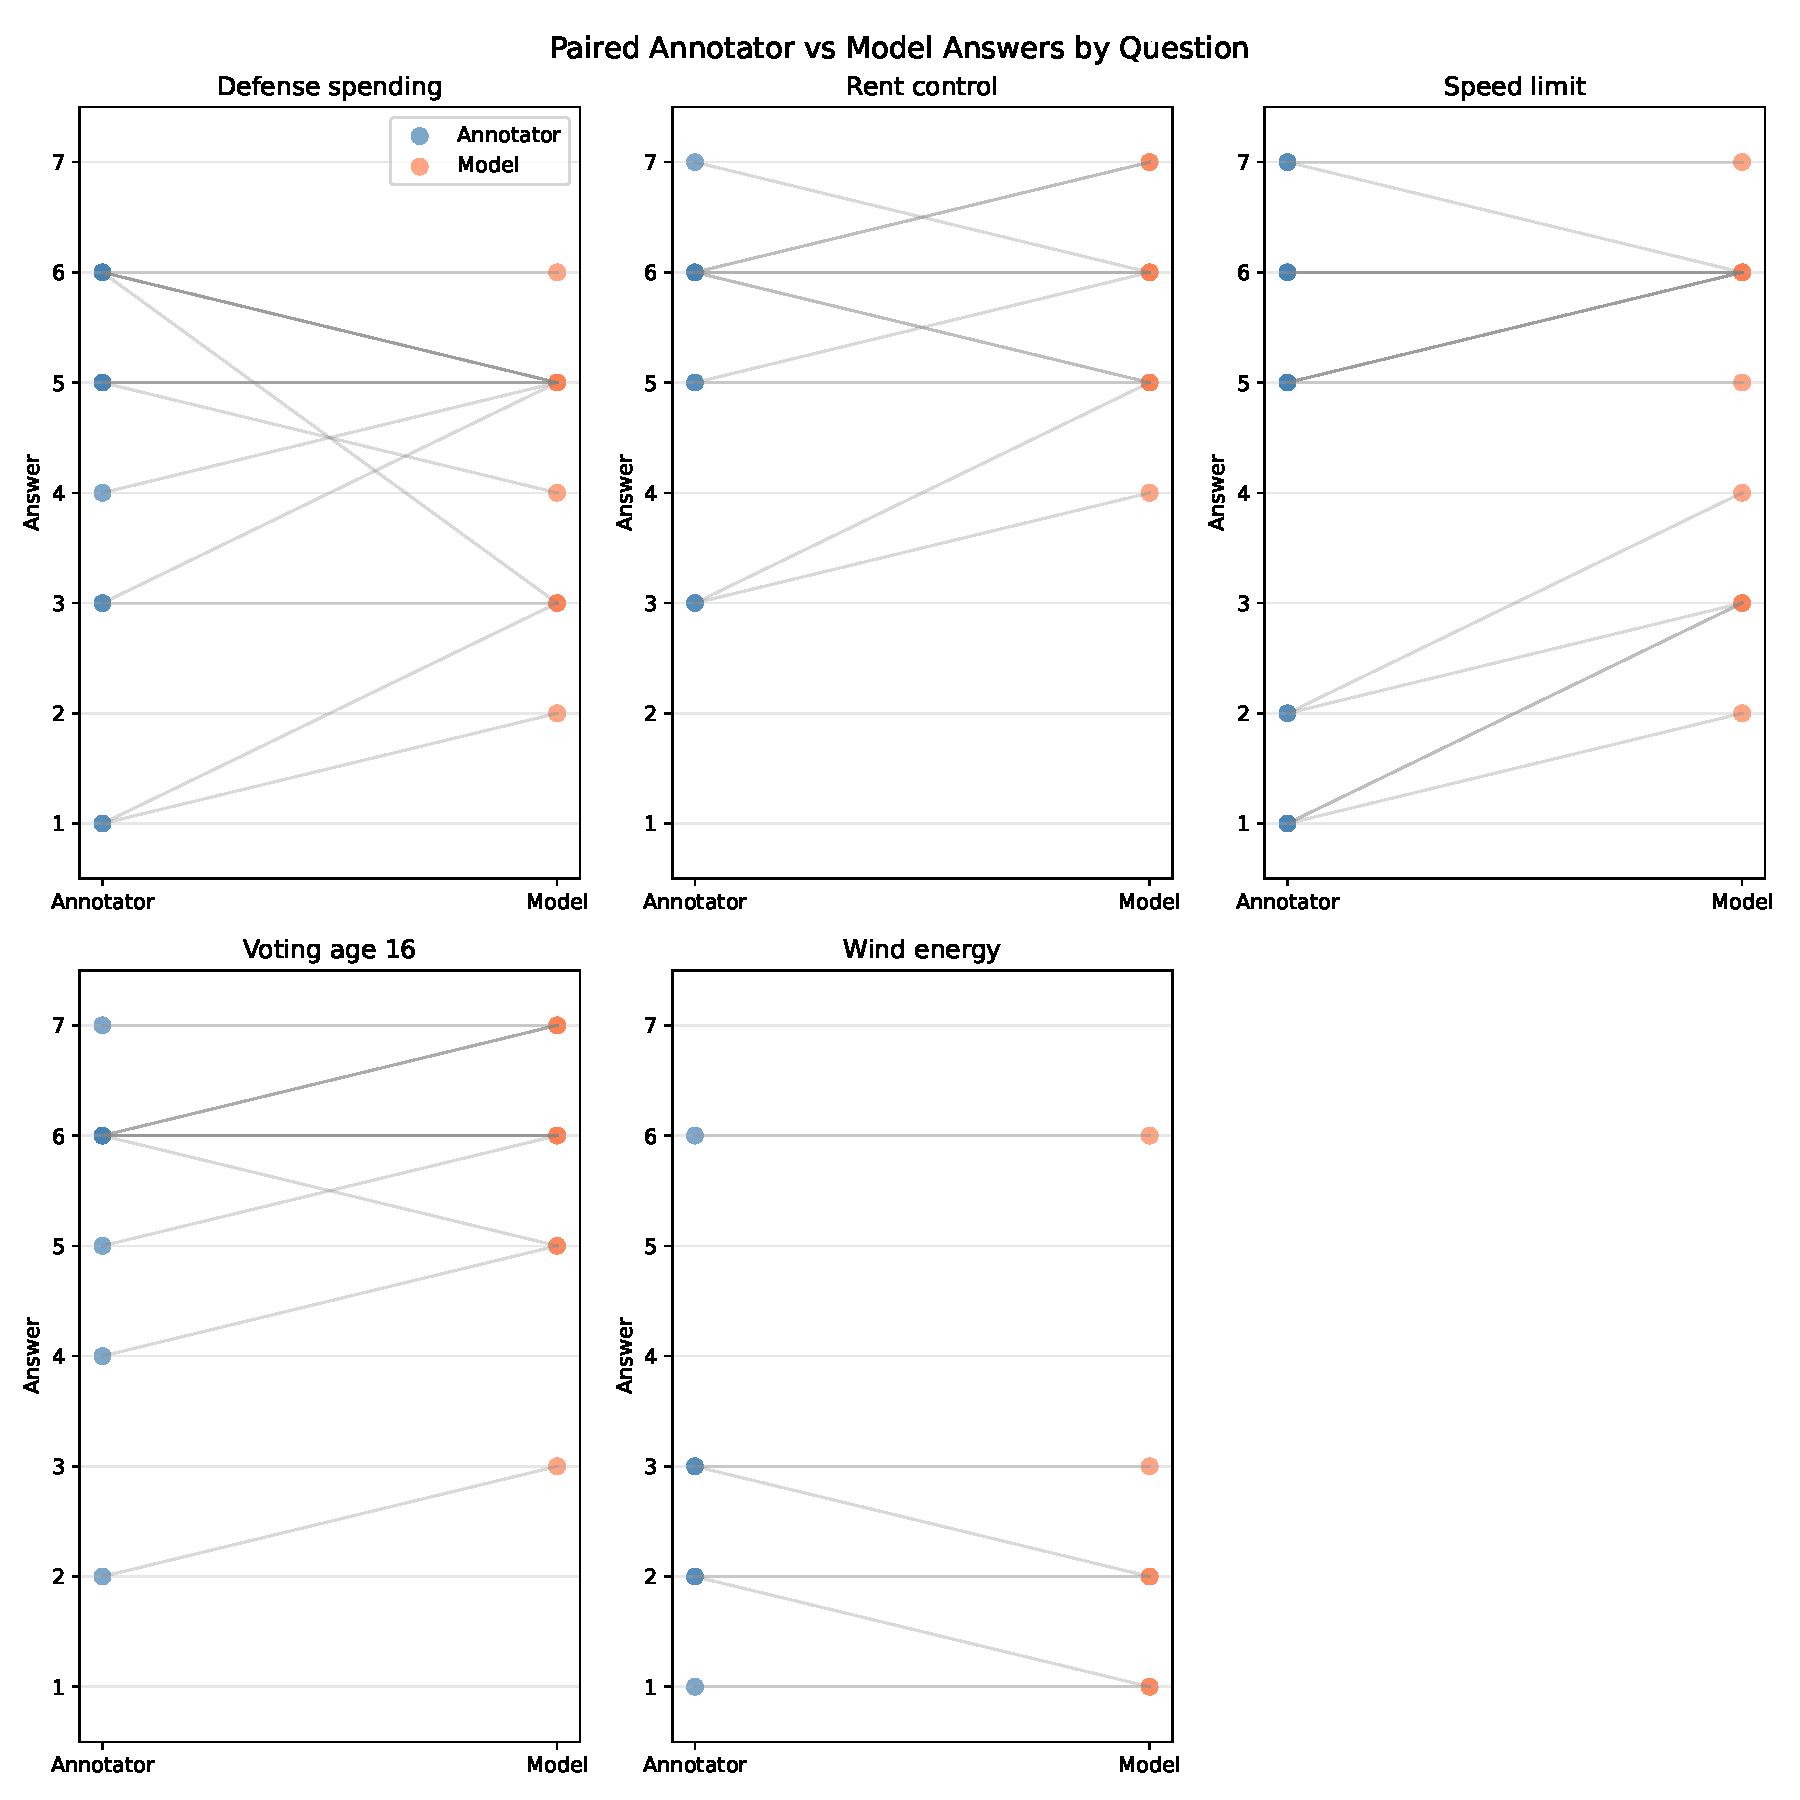
\includegraphics[width=\linewidth]{imgs/sanity_check_paired_plot.pdf}
\caption{Paired human and model ratings across questionnaire items. Lines connect corresponding observations; darker colours represent overlapping values.}
\label{fig:sanity_check}
\end{figure}


\section{Prompt Sensitivity - RQ1}


The Likelihood Ratio Test (LRT) was performed to compare the full model (Equation \ref{equ:full_model}) against the reduced model. The test yielded a highly significant result ($\chi^2(10) = 567.31, p < 0.0001$). This indicates that the model including the \texttt{prompt\_version} parameter provides a statistically significant better fit to the data than the model without it.

This finding confirms that the prompt phrasing has a significant influence on the agents' responses. Such sensitivity underscores the need for caution when designing experiments and interpreting results that rely on a single prompt version. This result supports our decision to employ a multi-prompt methodology, as it helps to mitigate potential biases introduced by any single phrasing.

It is important to note, however, that while this primary model showed a strong effect, two other models with different specifications were also analysed, and they yielded different results. This suggests the influence of prompt phrasing may be complex and potentially interact with other model assumptions, reinforcing the need for a robust, multi-prompt validation approach.

